
\newcommand{\tbi}[1]{$<$\textit{#1}$>$}

% Starts a new line nearly everywhere
\newcommand{\nl}{\mbox{}\\}
\newcommand{\nlskip}[1]{\mbox{}\\[#1]}

%
%Comments
\newcommand{\cmmnt}[1]{\framebox{#1}}
\newcommand{\bgcmmnt}[1]{\nl\framebox{\parbox{.95\textwidth}{#1}}\nl[2mm]}
%\renewcommand{\bgcmmnt}[1]{}
%

\newcommand{\eod}{\nl\rule{.95\textwidth}{1pt}\nl\textit{End of Document}}


\section{University of Bremen: Verification of the  Management of the Radio
Communication}
\label{sec:ubremen}
This section reports the verification activity of SCADE-MoRC. The goal
of this activity is, first, to establish the compliance of the SCADE
model to the SRS description via testing. Secondly, we want to track
the ambiguities within the specification. Finally we want to
demonstrate the efficiency of model based testing using the RT-tester
tool for system integration testing.

The activity is described in the Verification and Validation Plan
section {\em 6.1.2.7 System Integration Testing (Uni Bremen/DLR)} \cite{D4.1_2013}.
In short, we develop a test model from the specification, generate tests and use
the code generated from SCADE to perform software-in-loop testing.
The test model and the SCADE model used to generate code have been
done independently to each other. 

\paragraph{Object of verification}
 Management of radio communication (MoRC) ERTMS function baseline 3.


The system under test (e.g. the verification object) is the C code
generated from a SCADE model and described here
\url{https://github.com/openETCS/model-evaluation/tree/master/model/SCADE_Siemens/Subset_026_Chapt_3.5_ManagementOfRadioCommunication/Generated_C_Code}.
It describes the Management of the radio communication at the software
phase.




\paragraph{Available specification}

The specification is described in the
Subset-026 chapter 3.5. It
describes the communication protocol between the EVC and the RBC or
balises. In particular, how the EVC initiates and terminates a
communication.



\paragraph{Detailed verification plan}

\subparagraph{Goals}

To achieve what has been defined previously a test model in SysML has
been developed. The description of this verification artifact may be
found here \url{https://github.com/openETCS/model-evaluation/blob/master/model/EA-SysML/new_version/doc/ea_sysml_report.pdf}

Our main goal is to verify the SCADE model by test simulation. The
tests are produced by a model of the Subset-026 chapter 3.5 described as a
state machine.

\subparagraph{Method/Approach}

\begin{figure}
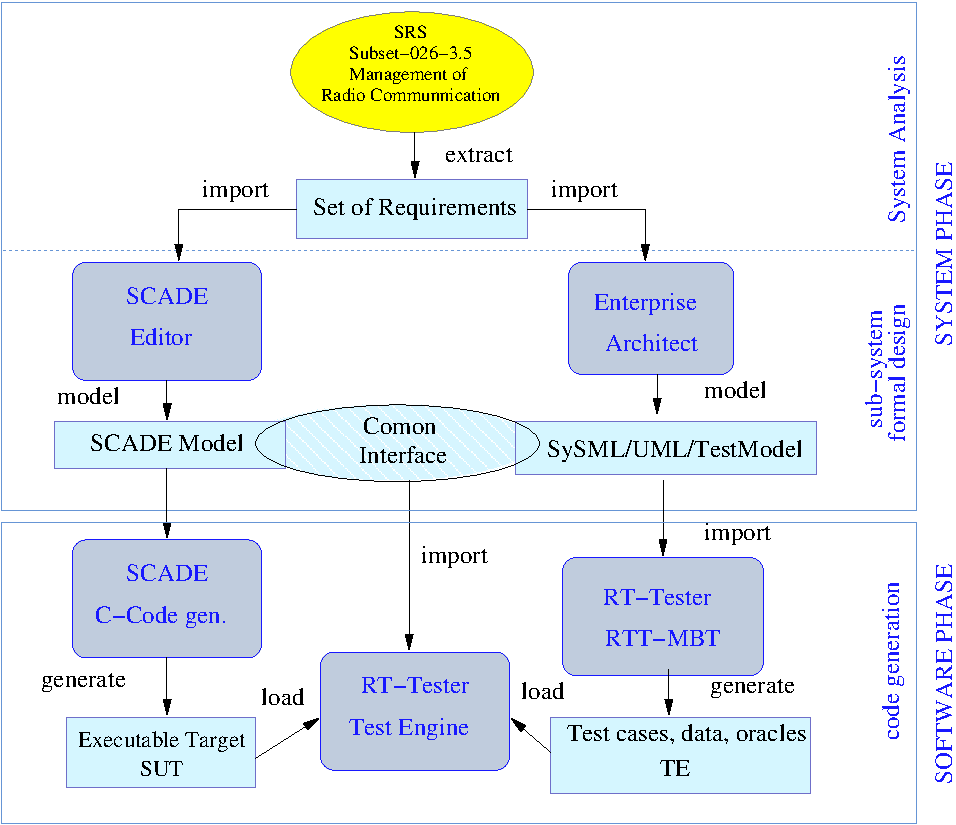
\includegraphics[width=\textwidth]{schema/framework}
\caption{\label{fig:method}SCADE/RT-Tester methodology}
\end{figure}

Figure \ref{fig:method} depicts our methodology. From the SRS
specification, two models are designed: one SCADE model that will
be then  used to produce C code and one SysML model for generating
tests.

Our test model contains the behavioral representation of the MoRC, the
set of requirements of the chapter 3.5, and the link between the behavior
and the requirement.  Most of the requirements may be represented as
single transition or state in the test model state
machine. Nevertheless, some of the requirements may be only modeled as
a path of the state machine, we choose to represent those as LTL
formula, added as constraints of the test model. For example the
\verb+REQ-3.5.3.10+ describes the steps needed for the establishment of
the radio communication order by the RBC. This requirement explicits a
particular path of the test model, thus this path should exists in our
test model. To ensure that this particular test will be generated a LTL
formula has been added (See \cite{braunstein_MorC_2013} for more
details).

\begin{description}
\item[REQ-3.5.3.10] "If the establishment of a communication session is
initiated by the RBC, it shall be performed according to the following steps
..."
\vspace{-1em}
\begin{verbatim}
Finally (MessageIn == INIT_SESSION_TRACK && setUp == 1 -> 
Next (MessageOut == SESSION_ESTABLISHED && radioComSession == ESTABLISHED)
\end{verbatim}
\end{description}

We need then to link the system under test and the test model. Since
the two models are elaborated independently, we need to ensure that
the tests generated may be handled by the code generated by SCADE and
conversely we need to read the output of the C code back to the test
generator to compare the values with our oracles. This is achieve by
defining a common interface that the two models should respect. The
inputs drive the tests and the outputs are the observational points to
state if a test pass or fail. Hence, the two models should respect the
same interface.

After the modeling phase, starts the test generation phase.
Two strategies have been used for the tests generation. First, we
generate a set of test following the common behavioral coverage
strategies ensuring the following coverage :
\begin{itemize}
\item  Basic control state coverage (BCS): All state locations are covered.
\item  Transition coverage (TC): All transition of the statecharts are covered.
\item  Modified condition/decision coverage (MC/DC): Modified condition/decision coverage.
\item  Hierarchic transition coverage (HITR): High-level transition of
  nested statecharts are covered.
\item  Basic Control states Pair coverage(BCPAIRS): For concurrent state
  machines pair states of two different state machines. 
\end{itemize}

More detailled explaination on the coverage may be found here \cite{huang_test_2013}.

We then apply a requirement coverage strategy to
generate tests that covers all the requirements. 
As each requirement
is linked to an artifact of the test model, part of the test cases
are generated as subset of the coverage mention above. In addition,
test cases from the LTL are also provided.


Finally the test engines run the SUT with the stimuli from the test
model. In parallel, it runs the test oracles that states if the test
pass or fail.

\subparagraph{Means}

The Artifacts are produced as follow:
\begin{itemize}
\item C code comes from SCADE model.
\item Test model is a SysML model designed with Enterprise Architect.
\item Test cases, tests data and test oracles are generated with RT-tester.
\item Executable code compile with gcc.
\item Code run within the RT-Tester engine.
\end{itemize}

SCADE is EN 50128 qualified at SIL 3/4, RT-tester is also certifiable
T3 as shown in \cite{peleska_efficient_2012}.

\subsection{Results}

\begin{table}[htbp]
\centering
\begin{tabular}{lr}\toprule
  Coverage strategies & \# tests generated  \\\midrule
  BCS & 14 \\
  TC & 40 \\
  MC/DC & 79 \\
  BCPAIRS & 33\\
  HITR & 12 \\
  LTL & 2 \\ \midrule
  Total Tests& 180\\\bottomrule
\end{tabular}

\vspace{1em}
%\raggedleft Total Requirements cover 40
\caption{\label{tbl:test_summary} Test cases generation summary}
\end{table}

Table \ref{tbl:test_summary} resumes the set of automatically
generated tests.
The set of tests cover 40 of the requirements from the chapter 3.5.


The simulation result of the C code is not yet finished and for the
moment, all test failed. The main reason was that the two
models did not share the same starting condition.
Hence, we  need to refined our test model to be able to handle SCADE
modeling style correctly and be able to have interesting result.



\paragraph{Summary}

What we have done:
\begin{enumerate}
\item Created a test model in SysML.
\item Generated test cases.
\item Ran SCADE model against test procedure produces by RT-tester.
\end{enumerate}
 
 The next step:
 \begin{enumerate}
 \item Refined test model
 \item Analyze the result of the test procedure.
 \item Coordinate DLR/SIEMENS/Uni Bremen interfaces.
 \item Run the test on the DLR lab.
 \end{enumerate}

\paragraph{Conclusions/Lessons learned}

Our first attempt to simulate the tests was not a success. All tests
except the one covering the initial states failed. Our two models
have, at least, the same initial state.
From  our first investigation, we could see that one chapter of
the specification is not self-contained. This leads to different
interpretation in the modeling and thus some non equivalent behaviors.

Moreover some missing information in the specification leads to 
 constraints in test model. It affects the test generation by
providing some non realistic test cases. Some variable behavior that
were not mentioned in the specification are considered as free and may have any
possible value in their definition range. This can be solved by adding
information into the test model. 

More precisely, the test model is composed with a system under test
and a test environment. In our first model the test environment is
empty, meaning that all inputs of the SUT are free. The test
enviroment may be described (and constrainted) by statecharts or
LTL formula that restricts the behaviors of the inputs. The test
generator should then find  test suites that realize the given
coverage and that respect the constraints given in the test environment.



\paragraph{Future Activities}
\subparagraph{Refine the test model}
\begin{enumerate}
\item Analyze the test results of the SCADE C code
\item Enumerates specification ambiguitites: where the two parties did
  not undestand the specification in the same way.
\item Refine the test model by adding a better test environment with
  the help of domain experts
\end{enumerate}
\subparagraph{New activities}
We will also provide the ceiling speed monitoring function to enrich
the test model and apply new model based testing approach.

%\bibliographystyle{plain}
%\bibliography{biblio}

